\chapter{Magnolia 5.0 technology stack}
\label{chapter_tech_stack}
\section{Overview}
As it was mentioned in the previous chapter Magnolia 5.0 will be dependent to the 
Vaadin and GWT frameworks. In addition a quite specific yet significant role is
dedicated to the JQuery library. In the current chapter we will provide some
clarification of the reasons for choosing such a set of technologies. The main
features of these frameworks will be observed as well.
\begin{figure}[H] \centering
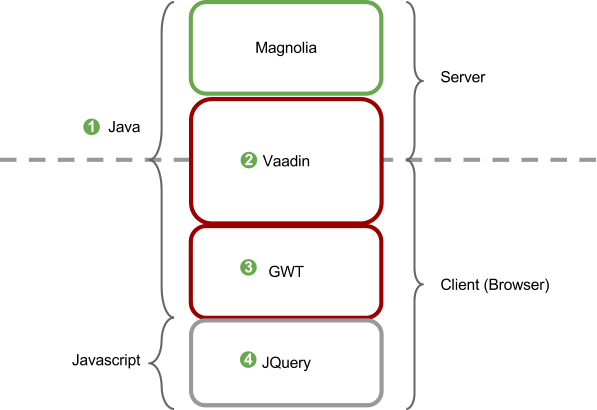
\includegraphics[width=\textwidth]{magnolia_stack.png}
	\caption{Magnolia CMS 5.0 technology stack}
	\label{fig:technology_stack}
\end{figure}

\section{A CMS vs an Application Framework}
First of all we should clarify the difference between a CMS and an application
framework. Most CMS's are built on top of an assumption about how the content
should be managed. Where as application frameworks make no assumptions about
that or even about what the content is. The power of an application framework is
in the set of basic capabilities it provides that allow to structure and manage
the data in any possible way. Magnolia 5.0 architecture proposal fits the
combination of two realms very well: while Magnolia core API's concentrate on
providing the best tools for website editors \cite{ux_andreas} let the
administration part of the CMS be built with an application framework that will
provide convenient ways to extend the system for developers. Such an approach
has a variety of benefits over the frameworks built in-house. First of all, this
would allow for adopting the best practices of application architecture design
by simply delegating the tasks to the application framework. The maintenance of
the system would be eased as well. The last but not the least benefit is the
smoother and easier adoption by Magnolia CMS community.

\section{Vaadin}
The Vaadin application framework is used for building the Magnolia 5.0
AdminCentral.
 
The core piece of the Vaadin Framework is the Java library designed to make
creation and maintenance of high quality web-based user interfaces easy. The key
idea in the server-driven programming model of Vaadin is that it lets you forget
the web and program user interfaces much like one would program any Java desktop
application with conventional toolkits such as AWT, Swing, or SWT \cite{BoV}.

As it is shown on the Figure \ref{fig:vaadin_arch} - the main part of Vaadin is
the server-side framework that runs within a Java application server on top of
the Java Servlet technology. A Vaadin application is stored in a servlet session
which typically handles the communication with various backend systems. An
Application also declares the user interfaces on the server side which are then
translated for different web browsers and rendered in the form of a JavaScript
program. The rendering and cross-compilation process of translating Java to
JavaScript is handled by GWT (a framework that we will discuss later on in this
chapter).

Being written completely in the Java language without and requiring no
additional configuration Vaadin integrates effortlessly with almost any other
Java technology. For example the dependency injection frameworks 
Spring and Google Guice. It also deploys deploys on almost any application server (e.g. JBoss,
GlassFish, Tomcat, Jetty etc). This means that Vaadin could easily be used with
Magnolia core API's out of the box.

Let us briefly study the architecture of the Vaadin framework.
\begin{figure}[H]
\begin{center}
  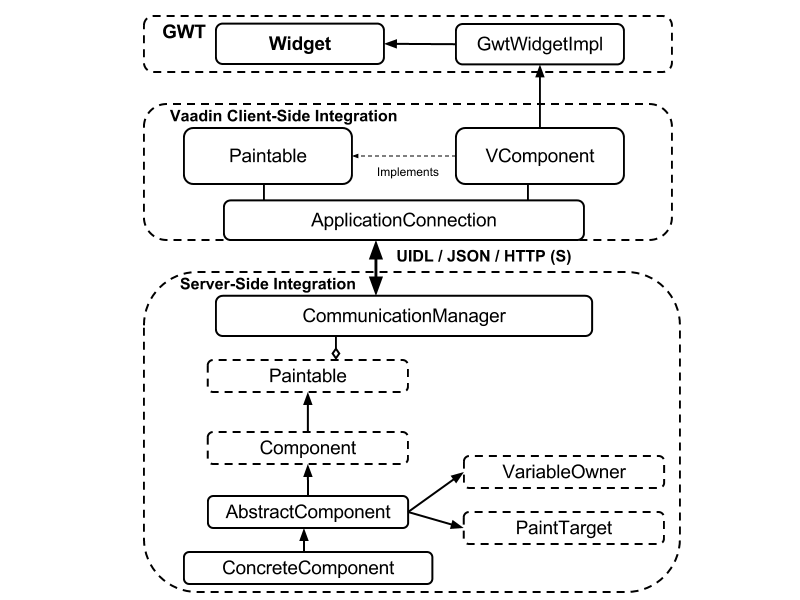
\includegraphics[width=\textwidth]{vaadin_architecture.png}
  \caption[labelInTOC]{Vaadin framework Architecture}
  \label{fig:vaadin_arch}
\end{center}
\end{figure}
 
\subsection{Servlet Level} 
An application that uses Vaadin runs as a servlet in a
Java web server, serving HTTP requests. The terminal adapter receives client
requests through the web server's Java Servlet API, and inteprets them to user
events for a particular session. Sessions are tracked using cookies. Events are
associated with UI components and delivered to the application, which handles
them with listeners. If the application logic makes changes to the server-side
UI components, the terminal adapter renders them in the web browser by
generating a response. The client-side engine running in the browser receives
the responses and uses them to make any necessary changes to the page in the
browser.

\subsection{Application level}.
The top level of a user application consists of an
application class that inherits \texttt{com.vaadin.Application}. It creates the
UI components (see below) it needs, receives events regarding them, and makes
necessary changes to the components.
For detailed information about inheriting the \texttt{Application} see \cite{BoV}.

\subsection{User Interface Components}
The user interface consists out of UI
components that are created and laid out by the application.
Each server-side component has a client-side counterpart, with which the user
interacts. The server-side components can serialize themselves over the client
connection using a terminal adapter. The client-side components, in turn, can
serialize user interaction back to the application, which is received in the
server-side components as events. The components relay these events to the
application logic. Most components are bound to a data source (see below). For a
complete description about the UI component architecture see \cite{BoV}.

\subsection{Client-Side Engine} The client-side Engine of Vaadin manages the
rendering in the web browser by using the Google Web Toolkit (GWT). It
communicates user interaction and UI changes to the server-side terminal adapter
by using the User Interface Definition Language (UIDL), a JavaScript Object
Notation (JSON) based language. The communications are made using asynchronous
HTTP or HTTPS requests.
\cite{BoV}.

\subsection{Terminal Adapter} Client-server communication in the Vaadin framework
is encapsulated into the so called Terminal Adapter concept. It is a mechanism
that typically manages the payload transfers between component client and server
counterparts while hiding the actual transport technology. Typically (in Vaadin
6) the underlying pipeline is the AJAX technology - the client side widgets fire
the events which are then transformed into variable changes by the
\texttt{com.vaadin.terminal.gwt.client.ApplicationConnection} class and sent to
server side where they are handled by the
\texttt{com.vaadin.terminal.gwt.server.CommunicationManager}. The
\texttt{CommunicationManager} class dispatches the changes to the corresponding
components which process them producing the response (the UIDL payload). As a
result the communication happens automatically and typically developers do not
have to take care about it unless they are building an extension for the Vaadin
framework.

\subsection{UIDL} The Terminal Adapter renders the user interface and its updates
to the Web page by means of the User Interface Definition Language (UIDL). The
UIDL communications are conducted over JavaScript Object Notation (JSON), which
is a lightweight data interchange format that is especially efficient for
interfacing with JavaScript-based AJAX code in the browser. \cite{BoV}.

\subsection{Events} User interaction with UI components creates events. The
lifecycle of an event typically starts with processing on the client side with
JavaScript. Then the event is passed all the way through the HTTP server,
terminal adapter, and finally - to the application instance and its user
component layers. \cite{BoV}.

\subsection{Themes} The user interface is a separator between presentation and
logic. While the UI logic is handled as Java code, the presentation is defined
in themes as Cascade Style Sheets (CSS). Vaadin provides a set of default
themes.
User themes can, in addition to style sheets, include HTML templates that define
custom layouts and other resources, such as images \cite{BoV}.
 

\subsection{Data Model} In addition to the user interface model, Vaadin provides
a data model for streamlining the data presented in UI components. By using the
data model, the user interface components can update the application data
directly, without the need for any control code. All the UI components use this
data model internally, but they can be bound to a separate data source as well.
For example, you can bind a table component to an SQL 
query response \cite{BoV}.In the case of the Magnolia CMS we will examine the
development of the \texttt{Container} implementation that binds to the Java Content
Repository.


\section{GWT}
Google Web Toolkit (GWT) is a development toolkit for building and optimizing
complex browser-based applications \cite{GWT}.
GWT is an open source framework developed by the Google corporation. The main
goal of the toolkit is to provide developers with an ability to write their
client side programs in Java without browser plugins or additional software.

\subsection{Compiler} 
The core of the Google Web Toolkit is a Java-to-JavaScript cross-compiler that
translates the Java program into highly optimized JavaScript code. The process
of cross-compilation involves the consequent building of Abstract Syntax Trees
(AST) that proceduraly formalizes Java code, optimizes it, translates to
JavaScript and then optimizes it again.
A possible drawback for the compiler is the time it requires to translate the
code. For a big projects this can take up to several minutes (even on powerful
machines with multi-core CPU's).

\subsection{Deferred Binding} 
Deferred binding is the crux of the GWT compiler. It is the process of
generating multiple chunks of JavaScript code each of which are later
served for different cases. The default case is the generation of different
versions of JS output (in order to overcome the browser dependent
peculiarities). It means that if some cases have to be handled differently e.g.
in FireFox and Internet Explorer, the developer does not have to use conditional
statements in his code but rather instruct the compiler on which logic to use
for each option. Such an approach reduces the amount of JavaScript code sent
over the network and improves code clarity and quality. Deferred Binding allows
for easier implementation of localization, resource handling and, what is very
important for Magnolia 5, automatic handling in cases of a visit from a mobile
devices\cite{def_bind}.

\subsection{JSNI}
Just like it is possible to inject C code into a Java program (Java Native
Interface or JNI) it is possible to inject the JavaScript code parts into the
GWT classes.

This approach brings many benefits for the GWT developers\cite{jsni}:
\begin{itemize} 
	\item Implement a Java method directly in JavaScript.
	\item Call from JavaScript code into Java code and vice-versa.
	\item Wrap type-safe Java method signatures around existing JavaScript.
	\item Throw exceptions across Java/JavaScript boundaries.
	\item Read and write Java fields from JavaScript.
	\item Use a development mode to debug both Java source (with a Java debugger) and JavaScript (with a script debugger).
\end{itemize}
In fact most of the low level GWT functionality is written with JSNI. It is
worth mentioning that irrational usage of JSNI can spawn a variety of issue like
more complicated portability across browsers, higher potential for memory leaks
than native GWT code and optimization issues \cite{jsni}. Nevertheless Magnolia
5.0 embraces it for integration of JavaScript libraries and API's and
development of widgets that would require more fine grained event handling.
[TODO - ADD CODE SNIPPETS AND EXPLANATION OF TYPE-MAPPING]

\subsection{Widgets and Events} 
The building block of GWT applications is the Widget
(\texttt{com.google.gwt.user.client.ui.Widget}).
Widget is typically a wrapper around a set of Document Object Model (DOM)
elements with business logic methods and event handlers. GWT is shipped with a
powerful event system which is based on the EventBus pattern. It allows for
building both user-defined events as well as the wrappers for the native DOM
events. GWT's event system carefully handles the cases with potential of memory
leaks \cite{gwt_memory_leaks} which are the source of various complex issue of
the programs written in plain Javascript. All this features are perfectly useful
for building readable and loosely coupled UI interfaces on the client side.

\section{JQuery}
JQuery is a popular JavaScript library which is so popular that it is probably
the first thing the name of the language is associated with. JQuery simplifies
HTML document traversing, event handling, animating, AJAX interactions and many
other areas of web development \cite{jquery}. 

JQuery is a base framework for a wide range of web project's front-end (e.g.
Wikipedia \cite{jquery}). However, in the case of Magnolia 5.0 project the
leading role in client-side development is devoted to GWT. Unfortunatelly, GWT
does not provide the solution for all the problems, a front-end developer might face.
One of such issues is a support for CSS3 transitions \cite{ccs3_transitions}.
Transitions API is not yet finally standardized and not fully cross-platform
which makes it hard to support with GWT. JQuery provides several convenient
approaches for adopting CSS3 transitions in the project. Due to \emph{JSNI}
mechanism it is possible to integrate JQuery with GWT and fulfill the gaps in
functionality of the latter. 
 
\section{Why Vaadin?}
\paragraph {Server Side Execution}
While execution of the UI events on the server side is quite controversial it
has several crucial benefits for a CMS development as CMS itself is mostly a
server side technology \cite{why_vaadin_philipp}.

\begin{itemize}
  \item Reflection can be used. While GWT code can't use reflection server side
  code can. This is for instance very helpful when 
  XML defined Magnolia entities are transformed into Java objects.

  \item Security is endorsed in many ways. Access Control Lists (ACL) can be
  easily used where ever needed. Additionally, having all the logic on the
  server side makes it next to impossible to break into the code and violate
  restrictions on the client side.

  \item Less web services. The UI is built on the server, but rendered on the
  client. So there is no need to define additional services for receiving dialog
  and tree descriptors. It is only required to expose the content related to the
  stateless Representation State Transfer (REST) services.

  \item Less GWT compilation is needed. Unless another module is added with its
  own client side implementation, the compilation should be done only once as to
  preserve development fluency. Agility is also increased by out-of-the-box
  support for any other JVM languages like Scala or Groovy. The latter of which
  is highly adopted in Magnolia.

  \item Testing concerns. Having all the logic on the server makes it easy to
  set up unit testing. Not only testing of for purely server side concepts like
  services, data storage connections and data processing, but also for testing
  of UI classes (to some certain extent). This is very important because, for
  instance, event handling in a complex application might become quite a fragile
  and sensitive task.
   
  \item Magnolia API. The Magnolia API can be fully exploited and no Data
  Transfer Objects (DTO) are required due to the fact that the UI logic is
  integrated with Magnolia API on the server side.

  \item Collaboration. The Magnolia and Vaadin communities and the backing
  companies are looking forward to support this collaboration and to help each
  other to make this successful.
  
\end{itemize}

\section{Possible Challenges}
The biggest cause of issues for the aforedescribed technology stack is the
performance. Being a server-side centristic application Magnolia 5 has to have
an architecture that finds a balance between a good and feature rich UI and
stable and scalable responsiveness. This could be described as several
requirements for the system:

\begin{itemize}
  \item Efficient data management. A proper integration of the JCR API and the
  Vaadin Data API is required. Due to memory consumption restrictions it is
  crucial that the smallest achievable amount of actual data is stored in memory
  at the same time. On the other hand, some caching or paging is needed in order
  to have most of the actual data accessible.
  
  \item [TODO: rephrase] Despite the fact that Vaadin has a big UI component
  bundle shipped with it - many of them have some sort of overhead:
  either rather complex DOM structure that is optimized for the versatility not
  crucial for considered project or too eager client-sever communication. This
  makes a demand for a row of additional components to be developed for Magnolia
  5.0 project.

  \item Transitions. Transitions between views is one of the key points of an
  interface optimized for good user experience. Smooth and logical transitions
  make the process of navigation more understandable and enjoyable. However,
  Vaadin does not support the transitions between the views out of the box.
  However, the existing solutions are server-side handled and they create an
  unnecessary communication spike on the back-end.
  
  \item Mobile support. Vaadin framework has an extension called the TouchKit
  which supposedly provides the functionality for mobile web applications.
  However, it was mainly created to support development of native-looking web
  applications and does not provide a framework with the capabilities for
  handling gestures and touch events. Thus, it is required to either build a new
  or integrate the existing solution to overcome this issue.
\end{itemize} 

\pagebreak
